%% LyX 2.2.3 created this file.  For more info, see http://www.lyx.org/.
%% Do not edit unless you really know what you are doing.
\documentclass[english]{article}
\usepackage[T1]{fontenc}
\usepackage[latin9]{inputenc}
\usepackage{amsmath}
\usepackage{graphicx}

\makeatletter
%%%%%%%%%%%%%%%%%%%%%%%%%%%%%% User specified LaTeX commands.
\date{}

\makeatother

\usepackage{babel}
\begin{document}

\title{Pictures with basic description\\
on \\
\textbf{Kuramoto-Model Coupling Reconstruction Process}}
\maketitle

\section{General scope of the reconstruction procedure and used notation}

In this part of the current paper we provide the description of Kuramoto
model, notation for used variables and general description of inverse
problem for Kuramoto model being studied.

Let us consider two oscillators with frequiences $\omega_{1}$ and
$\omega_{2}$ respectively; let $\Omega=\frac{\omega_{1}+\omega_{2}}{2}$
be their sychronised common frequency, thus 
\[
\begin{cases}
\omega_{1} & =\Omega+\Delta\omega\\
\omega_{2} & =\Omega-\Delta\omega
\end{cases},
\]
where we denote symmetrical frequency difference as $\Delta\omega$.
In order to describe the evolution of their phases $\theta_{1}(t)$
and $\theta_{2}(t)$ we propose following diffrential equations(let
us denote the coupling function of oscillators as $k=k(t)$):
\[
\begin{cases}
\dot{\theta}_{1}=\omega_{1}+\frac{k}{2}\sin\left(\theta_{2}(t)-\theta_{1}(t)\right)\\
\dot{\theta}_{2}=\omega_{2}+\frac{k}{2}\sin\left(\theta_{1}(t)-\theta_{2}(t)\right)
\end{cases},
\]
which could be easily transformed by summing and substracting equations
above into the following:
\[
\begin{cases}
\dot{\theta}_{1}+\dot{\theta}_{2}=2\Omega\\
\dot{\theta}_{1}-\dot{\theta}_{2}=2\Delta\omega-k\sin\left(\theta_{1}(t)-\theta_{2}(t)\right)
\end{cases}
\]

Denoting $\theta=\theta_{1}-\theta_{2}$, we get 
\begin{equation}
\dot{\theta}=2\Delta\omega-k\sin\theta(t)\label{eq:kur1}
\end{equation}
Solving equation (\ref{eq:kur1}), the evolution of phaze difference
can be obtained (assuming the first equation of the system is easily
solvable); this states the direct problem in Kuramoto model.

Our paper focuses on the \emph{inverse} problem: considering that
the coupling $k(t)$ is generally unknown, let us assume that its
approximation $k_{0}(t)$ can be obtained from the real data (the
whole procedure of its extraction and neccesary assumptions are not
in the scope of this report). Then by solving equation (\ref{eq:kur1})
with $k=k_{0}(t)$ we get the approximation of phaze difference $\theta_{0}(t)$;
this can be use to construct two ``virtual'' oscillators with given
phaze difference $\theta_{0}(t)$:
\[
\begin{cases}
X_{0}(t)=\sin\left(\Omega t\right)\\
Y_{0}(t)=\sin\left(\Omega t+\theta_{0}(t)\right)
\end{cases}
\]
Note that proposed virtual oscillators imply that amplitudes of both
oscillators are the same; moreover let us compute the sliding correlation
$C_{0}(t)$ between $X_{0}(t)$ and $Y_{0}(t)$ over a window of common
period of oscillators $T=\frac{2\pi}{\Omega}$:
\begin{align}
C_{0}(t) & =C_{T}(X_{0},Y_{0})=\label{eq:slide}\\
 & =\frac{\int_{t-T/2}^{t+T/2}\left(X_{0}(\tau)-\left\langle X_{0}(\tau)\right\rangle _{T}\right)\left(Y_{0}(\tau)-\left\langle Y_{0}(\tau)\right\rangle _{T}\right)d\tau}{\sqrt{\int_{t-T/2}^{t+T/2}\left(X_{0}(\tau)-\left\langle X_{0}(\tau)\right\rangle _{T}\right)^{2}d\tau\int_{t-T/2}^{t+T/2}\left(Y_{0}(\tau)-\left\langle Y_{0}(\tau)\right\rangle _{T}\right)^{2}d\tau}},\nonumber 
\end{align}
where by $\left\langle X_{0}(\tau)\right\rangle _{T}$ we denote the
mean value of $X_{0}(t)$ over used window.

The main assumption of overseen reconstruction procedure states that
the system is close to its stationary state; in which case the sliding
correlation between oscillators can be computed as $\theta_{0}(t)=\cos C_{0}(t)$.
So in case of quasi-stationarity new reconstructed phaze difference
$\varphi(t)$ can be obtained using $C_{0}(t)$ computed by eqaution
(\ref{eq:slide}):
\[
\varphi(t)=\arccos C_{0}(t)
\]
Using that $\dot{\varphi}\approx0$ one could substitute $\theta$
with $\varphi$ in the equation (\ref{eq:kur1}) and find reconstructed
coupling $\hat{k}(t)$:
\[
\hat{k}(t)=\frac{2\Delta\omega}{\sin\varphi(t)}
\]

Note that described procedure is proved to be correct in case
\begin{equation}
\left|k_{0}(t)\right|\ge2\Delta\omega\label{eq:ineq}
\end{equation}

which is refered as \emph{the main Kuramoto inequality}.

\section{Model functions and reconstruction}

In this part of our research we investigate the proposed reconstruction
procedure from qualitative and quantitative (we describe used metrics
further) points of view for 4 different sets of coupling approxiamtions
$k_{0}(t)$: piecewise-constant, sine, autoregressive approximations
and its combination; focusing on the case of temporarily breaking
the main Kuramoto inequality (\ref{eq:ineq}).

\subsection{Piecewise-constant approximations}

In this case we assume that $k_{0}(t)$ can be described as
\[
k_{0}(t)=\begin{cases}
d, & t<T_{0}\lor t>T_{0}+s\\
d+\Delta d, & T_{0}\le t\le T_{0}+s
\end{cases}
\]
where $\Delta d$ can be either positive or negative; we refer to
the period of the second value $d+\Delta d$ as the shock period.

\begin{figure}[!h]
\centering{}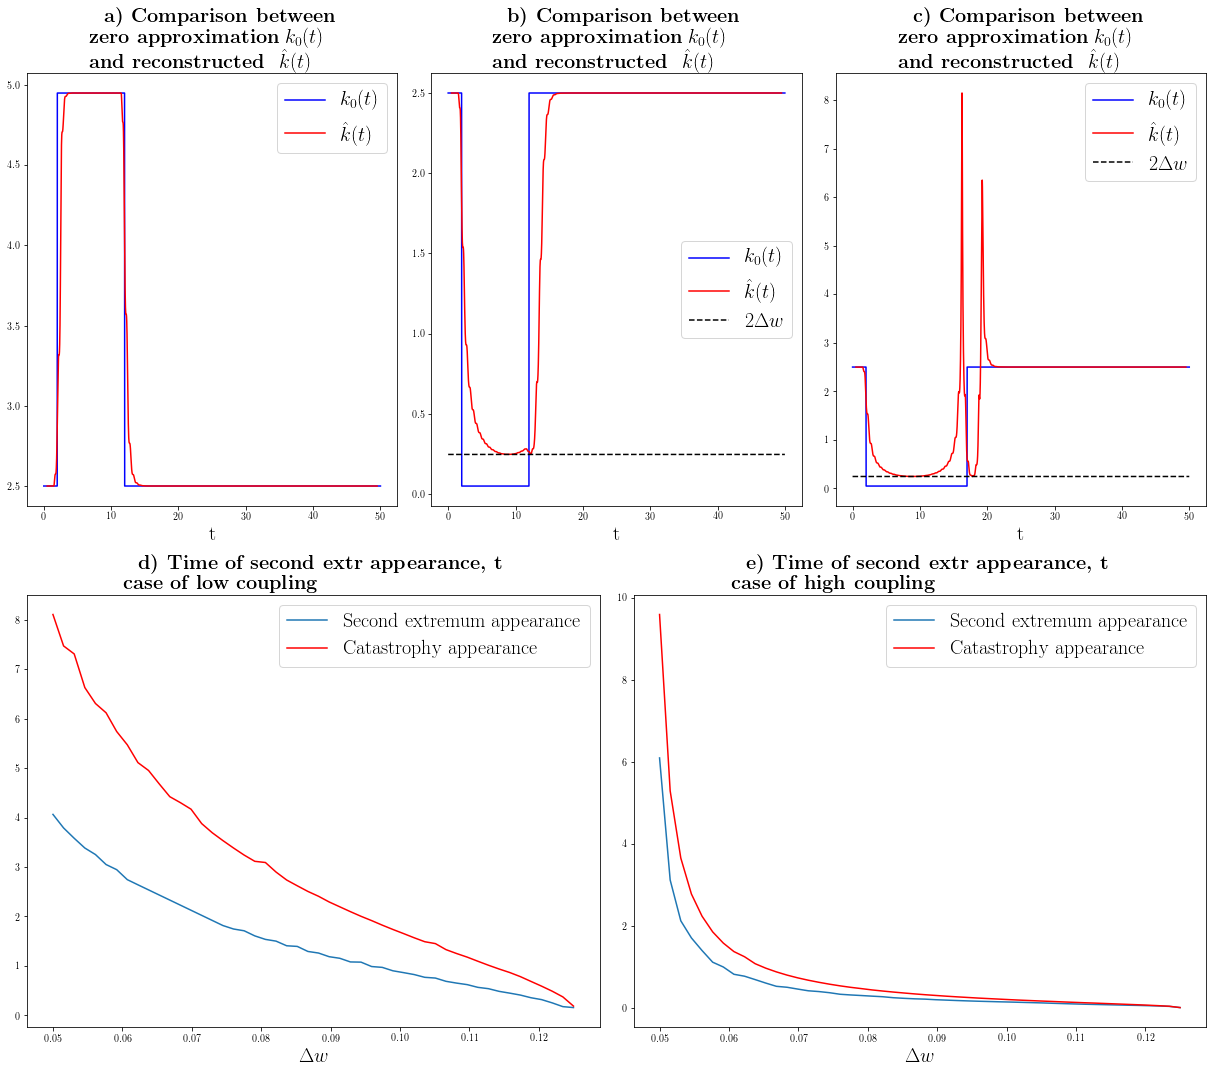
\includegraphics[width=1\textwidth]{../../python/pics/v2/constv2}\caption{Reconstruction of piecewise-constant aprroxiamtion $k_{0}(t)$: examples
and length of the period with shock corresponding to the second extremum
and singularity appearances\label{fig:pc}}
\end{figure}

Figures (1a\textendash c) illustrate results of reconstruction of
single approximation in three different cases: without breaking the
main Kuramoto inequality (1a); breaking Kuramoto inequality with resulting
additional extremum appearance after the shock period (1b); and breaking
Kuramoto inequality with resulting appearance of singularity in reconstructed
function (1c). 

In case of (1a) it can be seen that the system relaxes to the shocked
value during the shock period and to the normal value after the shock
significant amount of time (measured in common period of oscillators);
thus one can say that the system has a noticible ``memory''. As
for the effects of breaking the main Kuramoto inequality (among cases
in which the shock period is not long enough to create qualitatively
new figures) we outline two different scenarious: if the shock period
is long enough (consider figures (1d\textendash e) in order to established
the appropriate length) reconstructed function tends to begin a relaxation
to the normal value even before the shock period is over thus creating
the second extremum after the shock; in case when the system has enough
time to fully relax to the normal value during the shock, the reconstruction
process results into the singularity in $\hat{k}(t)$ (specifically
this means that in that moment of time oscillators are fully uncorrelated). 

For the further investigation of this phenomena we provide figures
(1d\textendash e) devoted to establishing the length os the shock
period $s$ towards $\Delta\omega$ sufficient for the second extremum
and singularity; to give more sophisticated picture we study cases
of low coupling (low $d$, comparatively two $2\Delta\omega$) (fig.
1d) and high coupling (fig. 1e). As shown increasing (and therefore
strengthing the breaking difference in the inequality) symmetrical
phaze diffrenece results into earlier appearance of both effects.

\subsection{Sine approximations}

In this part we propose coupling approximation as follows:
\[
k_{0}(t)=A\sin\left(Bt+\varepsilon\right)+C,
\]

where $A$ is an amplitude, $B$ is a frequency and $C$ is a mean
value. Moreover, consider $C-A<2\Delta\omega$, so we study only the
case of inequality breaking.

\begin{figure}[!h]
\centering{}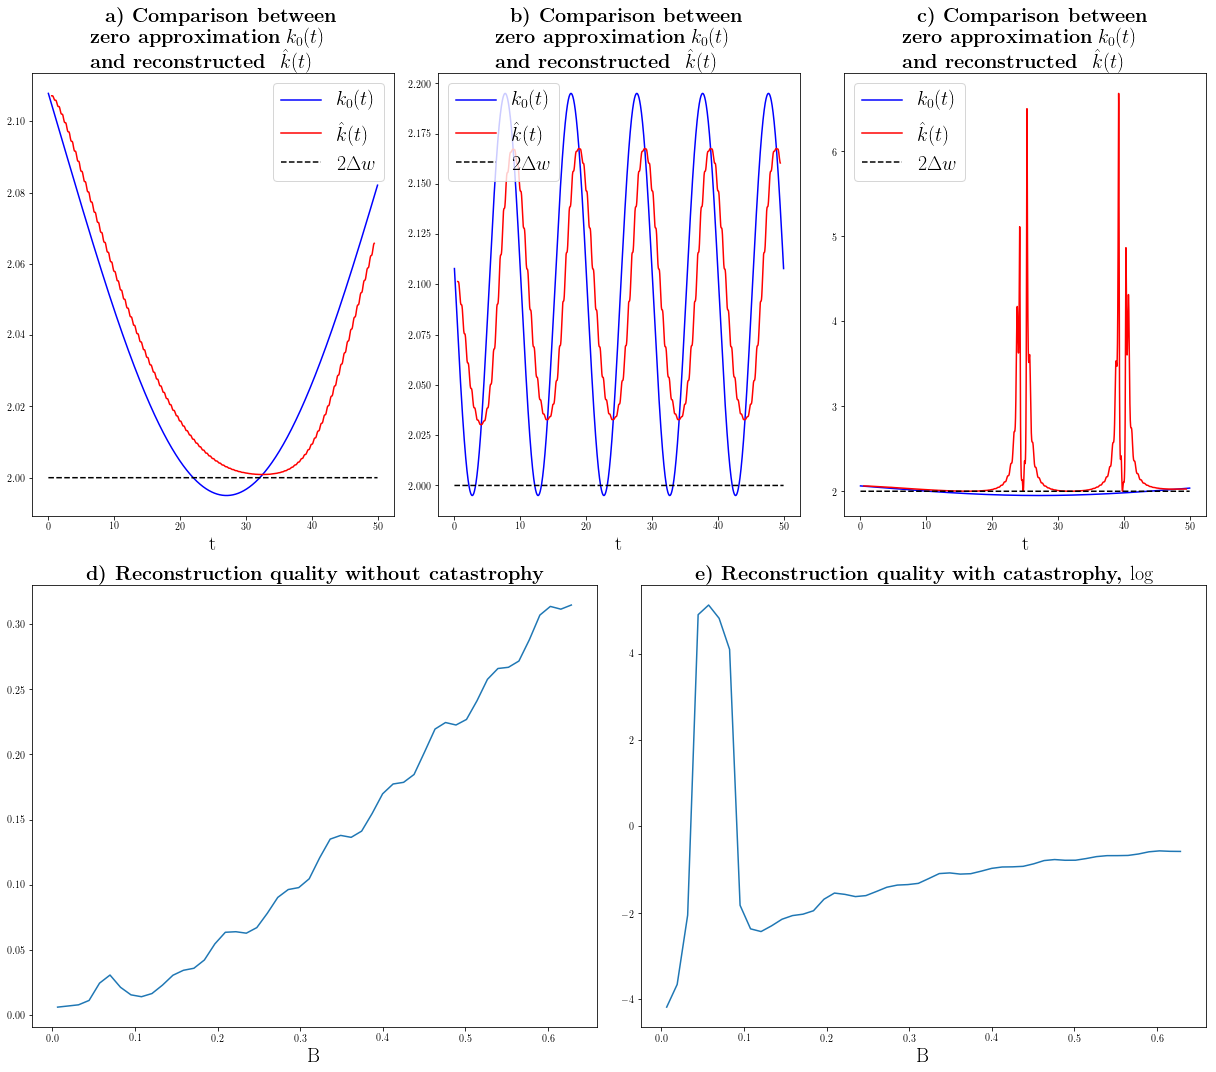
\includegraphics[width=1\textwidth]{../../python/pics/v2/sinv2}\caption{Sine approximations of $k_{0}(t)$: examples and quality of reconstruction
towards sine frequency\label{fig:sin}}
\end{figure}

Same as for piecewise-constant case, figures (2a\textendash c) illustrate
results of reconstruction of single approximation; for those pictures
we vary the frequency of sine being reconstructed. Figure (2a) shows
the case for correct reconstruction despite the inequality breaking;
similar to the piecewise-constant case (fig. (1b)) we observe gradual
relaxation to restrcited by inequality values with noticible flatenning.
Figures (2b) and (2c) shows two opposite cases of poor recontruction
quality: for the figure (2b) it can be seen that more frequent fluctuation
are less appropriate for reconstruction which can be explained not
sufficient time for relaxation seen on fig. (1) and (2a); figure (2c)
shows the case of singularity achieved by the same condition as on
fig. (1c) \textemdash{} too long restricted value period.

Figures (2d\textendash e) generalize the study of reconstruction towards
sine frequency; to measure the quality of the process we propose the
following metric:
\[
R_{0}[\hat{k},k_{0}]=\frac{\int_{0}^{L}\left(k_{0}(t)-\left\langle k_{0}(t)\right\rangle _{L}\right)\left(\hat{k}(t)-\left\langle \hat{k}(t)\right\rangle _{L}\right)dt}{\int_{0}^{L}k_{0}^{2}(t)dt}
\]
Figure (2d) illustrates the case of $C-A>2\Delta\omega$; thus general
increase of error corresponds with phenomenon observed on fig. (2b).
Figure (2e) explores the case of $C-A<2\Delta\omega$ (in log scale):
here we can see three different parts \textemdash{} the first one
corresponds with the case of no breaking (such as fig. (2d)), then
we obtain highly unreconstructed part corresponding to fig. (2c),
and finally we get similar to fig. (2d) line explained by increase
of sine frequency.

\subsection{Autoregressive ramdom approximations}

In order to simulate the random noise for our procedure we study autoregressive
process (AR(1)), which can be described as:
\[
k_{0}(t_{n})=\alpha k_{0}(t_{n-1})+\xi_{n},
\]

where $\xi_{n}\sim\mathcal{N}(\mu,\sigma)$ and $\alpha<1$. This
stochastic process is widely on as weakly stationary after $n=\frac{1}{1-\alpha}$
with the mean equal to $\frac{\mu}{1-\alpha}$ and standart deviation
equal to $\frac{\sigma^{2}}{1-\alpha^{2}}$.

\begin{figure}[!h]
\centering{}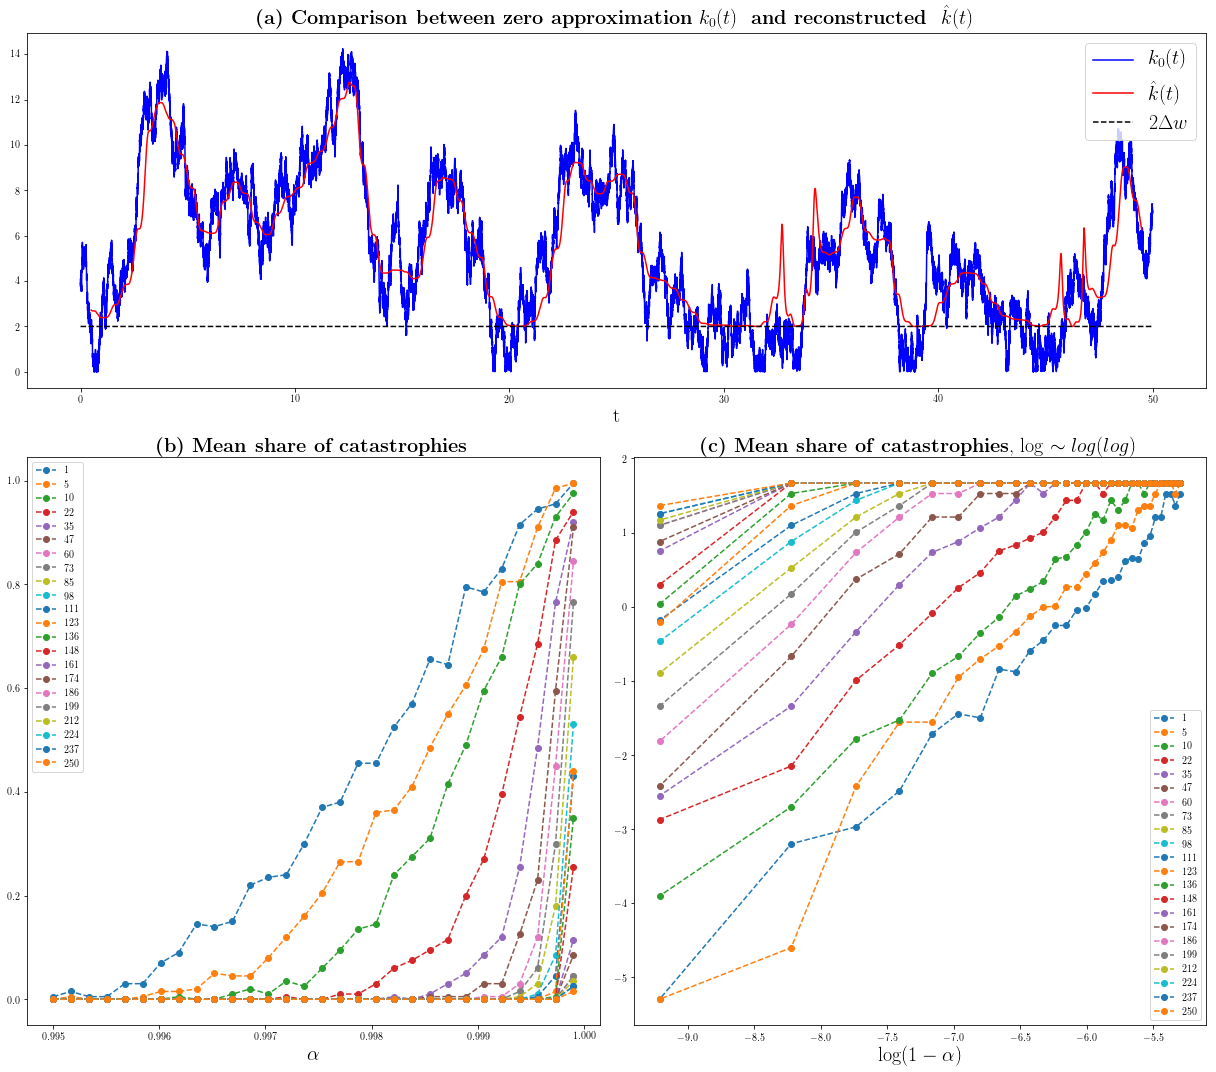
\includegraphics[width=1\textwidth]{../../python/pics/v2/ar1v2}\caption{pampam}
\end{figure}

One realization of described process is shown of figure (3a). According
to the stochastic character of the process one shoule assume that
for every set of parameters all seen for previous functions cases
of reconstruction are possible with some probability. Thus we vary
$\alpha$ and $\mu$ on figure (3b\textendash c) in order to get probability
of singularity in this case.

\begin{figure}[!h]
\centering{}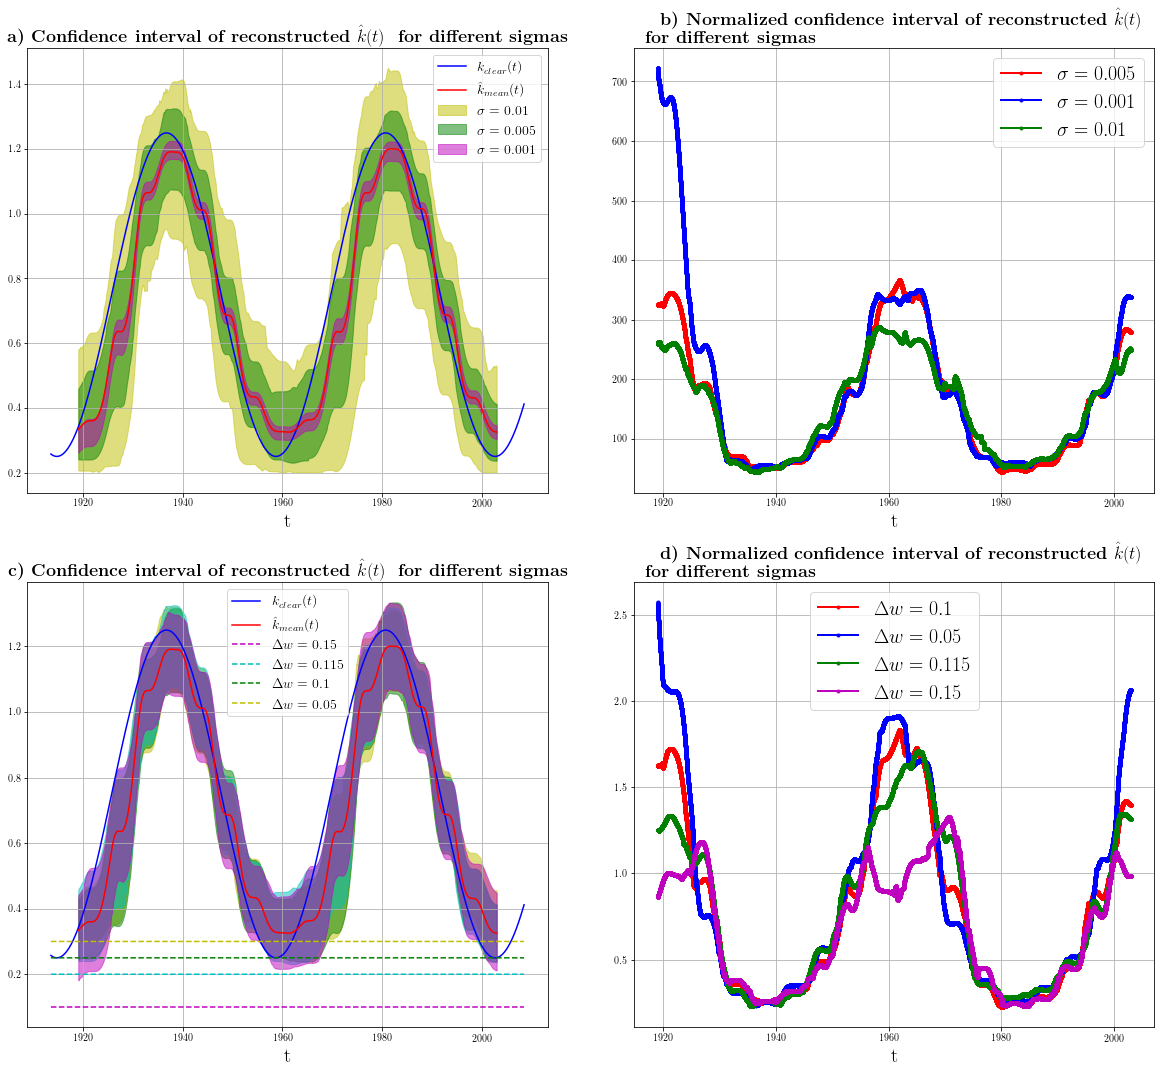
\includegraphics[width=1\textwidth]{../../python/pics/v2/civ2}\caption{pampam}
\end{figure}

\end{document}
